\section{Aufbau und Durchführung des Versuchs}
\label{sec:Durchführung}
Die Messung wird mit dem in Abbildung \ref{fig:app} zu sehenden D8-Diffraktometer durchgeführt. 
Bei diesem handelt es sich um eine Röntgenröhre mit einer Kupferanode welche mit einer Spannung von $\SI{40}{\kilo\volt}$
und einem Strom von $\SI{40}{\milli\ampere}$ betrieben wird. \\
\begin{figure}[H]
  \centering
  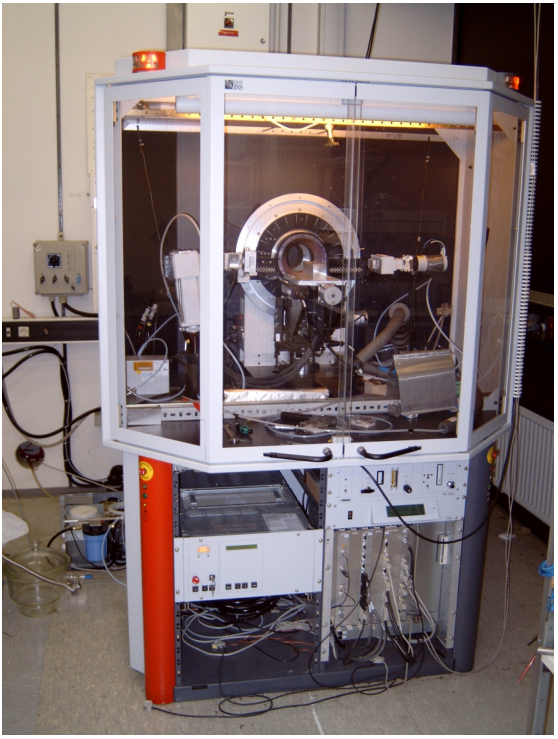
\includegraphics[width=0.4\textwidth]{content/images/apparatur.PNG}
  \caption{Das verwendete D8-Labordiffraktometer \cite{anleitung}. }
  \label{fig:app}
\end{figure}
Die aus der Röntgenröhre divergierende Strahlung wird hier mithilfe eines Göbelspiegel
gebündelt und monochromatisiert. Der daraus resultierende Strahl besitzt dann eine Wellenlänge von
$\lambda=\SI{1.54}{\angstrom}$. Ein Bild der verwendeten Röntgenröhre befindet sich in Abbildung \ref{fig:anode}.

\begin{figure}[H]
  \centering
  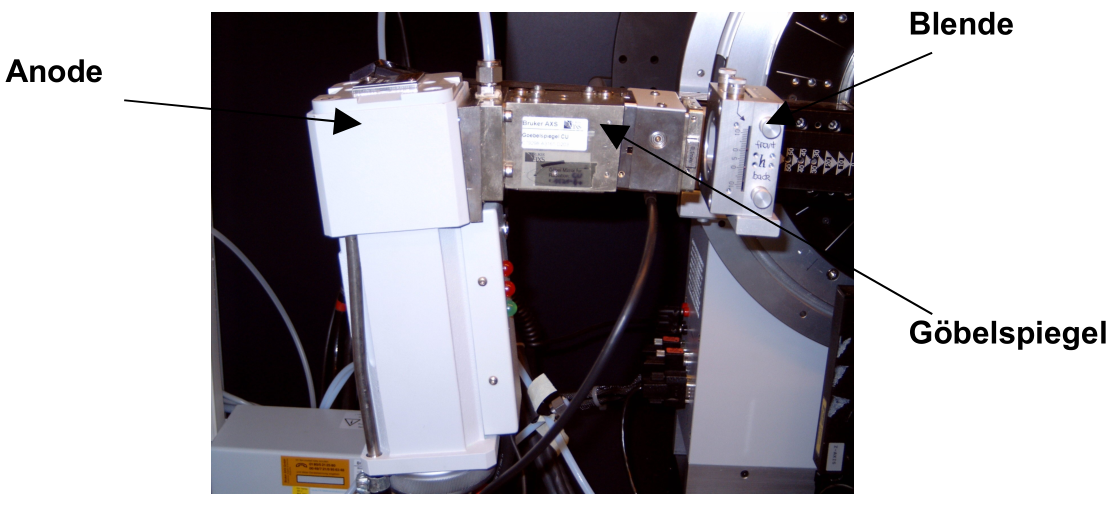
\includegraphics[height=4cm]{content/images/anode.PNG}
  \caption{Röntgenröhre des D8-Labordiffraktometers\cite{anleitung}.}
  \label{fig:anode}
\end{figure}

%Mit Hilfe des Gerätes kann sowohl der Winkel der Röntgenröhre, als auch der Winkel des Detektors zum Probentisch
%genau eingestellt werden. Desweiteren ist es
%möglich den Probentisch in x-, y- und z-Richtung zu fahren.
%Die Abbildung \ref{fig:anode_det} enthält zum Einen eine genaue Ansicht auf die
%Röntgenröhre mit Blende und zum Anderen auf den Detektor des Gerätes.


\subsection{Justage}
\paragraph{Detektorscan}
Um den Detektorscan durchzuführen, wird zunächst die Probe aus dem Strahlengang entfernt. 
Dabei werden Röntgenröhre und Detektor so zueinander eingestellt,
dass sie einen Winkel von $\SI{0}{\degree}$ einschließen. Um nun die tatsächliche Nulllage des Detektors zu finden, wird seine Lage um wenige Grad varriert, bis die Intensität des Primärstrahles ein durchläuft Maximum durchläuft, welches für die folgenden Schritte als neue Nullposition des Detektors verwendet wird. 

%  Z-Scan #1
\paragraph{Erster Z-Scan}
In diesem Schritt wird die Probenjustage angepasst. Dabei wird die z-Position der Probe varriert. Dazu wird diese wieder in den Strahlengang geschoben und die Intensität $I$ gemessen. Ziel dieser Messung ist es, herauszufinden, wann dabei die gemessene Intensität $I$ auf $\frac{1}{2} I_\text{Max} $ sinkt. Der z-Wert wird notiert und die Motoren in die entsprechende Position gebracht. 

% Rocking-Scan 0 grad
\paragraph{Erster Rockingscan}
Nachdem in den vorherigen Schritten die zu untersuchende Probe parallel zur Strahlachse ausgerichtet wurde, erfolgt nun der Rockingscan. Bei diesem Röntgenröhre und Detektor um die Probe bewegt, wobei der Winkel zwischen Detektor und Probe bei Konstant $2\Theta = \SI{0}{\degree}$ bleibt. Die Drehung erfolgt dabei im Winkelbereich zwischen $\SI{-1}{\degree}$ und $\SI{1}{\degree}$. Aus dem daraus folgendem Intensitätsverlauf wird das Maximum ausgelesen und für die weiteren Schritte verwendet. 

% Z-Scan #2
\paragraph{Zweiter Z-Scan}
Die Probe befindet sich aufgrund des Rockingscans nun nicht mehr in der Position, in der die gemessene Intensität $I$ der halben maximalen Intensität $\frac{1}{2} I_\text{Max} $ entspricht. Aus diesem Grund muss hier ein erneuter Z-Scan durchgeführt werden. 



% Rocking-Scan 0.3 grad
\paragraph{Zweiter Rockingscan}
Zur Erhöhung der Präzission wird nun ein zweiter Rockingscan mit $2\Theta = \SI{0.3}{\degree}$ durchgeführt. Dabei wird für die Drehung ein Winkelbereich
von $\SI{0.1}{\degree}$ bis $\SI{0.2}{\degree}$ gewählt.


% Z-Scan #3
\paragraph{Dritter Z-Scan}
Um die Präzission der Justage weiter zu erhöhen, wird anschließend ein dritter z-Scan bei $2\Theta = \SI{0.3}{\degree}$ durchgeführt. Dabei wird ein Scanbereich zwischen $\SI{-0.5}{\milli\meter}$ und $ \SI{0.5}{\milli\meter}$ gewählt. Wie auch bei den vorherigen z-Scans wird hier erneut das Maximum gemessen und die Motoren entsprechend angesteuert.

% Rockingscan 1.0 grad
\paragraph{Dritter Rockingscan}
Als letzter Schritt wird ein abschließender Rockingscan unter einem Winkel von $2\Theta = \SI{1}{\degree}$ durchgeführt. 
Dabei wird ein Scanbereich zwischen den Werten $\SI{0.45}{\degree}$ und $\SI{0.55}{\degree}$ gewählt, da das erwartete Maximum bei $\SI{0.5}{\degree}$ liegt.
Nachdem das Maximum gefunden wurde, werden die Motoren entsprechend angesteuert. 



\subsection{Messung}
\label{subsec:messung}
Nachdem die Justage des D8-Diffraktometer durchgeführt wurde, wird ein sogenannter Reflektivitätsscan durchgeführt. Bei diesem sind der Einfallswinkel $\alpha_i$ und der Winkel zwischen Probe und Detektor $\alpha_{\text{f}}$ gleich. Im verwendeten wird hierbei ein Scanbereich von $\SI{0}{\degree}$ bis
$\SI{5}{\degree}$ eingestellt und vermeessen. Dazu wird eine Schrittweite $\SI{0.05}{\degree}$ verwendet, wobei als Messzeit pro Datenpunkt $\SI{5}{\second}$ gewählt wird. \\
Zusätzlich wird ein sogenannter diffuser Scan durchgeführt, der den Anteil der gestreuten Intensität an der Reflektivität bestimmt. Dieser Scan wird mit dem Unterschied durchgeführt, dass die Differenz hier $\Delta a = | \alpha_i - \alpha_{\text{f}} | =  \SI{0,1}{\degree} $ beträgt.
